\documentclass[12pt,a4paper]{report}
\pdfminorversion=7
\usepackage[pdftex]{graphicx}

\begin{document}
\begin{titlepage}
Data Master Test Description

22.4.2020

Martin Skorsky
\end{titlepage}

\chapter{Introduction}
Currently there are 9 automated tests for the data master. The tests are driven by a Python script \texttt{dm\_testman.py}.

The static tests just add and remove patterns. The dynamic test in addition start the patterns.
\section{How to run the tests}
(ToDo)
\section{Prerequisites}
This test framework requires Python 3.6m or higher. A data master has to be accesible from the host. 
The source for the tests is at 

Project: \texttt{https://github.com/GSI-CS-CO/bel\_projects/},

Path: \texttt{modules/ftm/ftmx86/full\_test/}.

For each test the data master is halted and cleared. All patterns are removed.

\chapter{Description of Tests}
\section{Structure of Description}
\begin{enumerate}
	\item Purpose of Test

	What is the objective of this test?
	\item Prerequisites of Test

	What is the setting of the test?
	\item Test Actions

	List the actions of the test. This includes the graphs of the test pattern.
	\item Success Criteria

	What is checked to state a successful test?
\end{enumerate}
\section{Static Tests}
\subsection{Basic}
\begin{enumerate}
	\item Purpose of Test

	This test uses \texttt{dm-sched add} and \texttt{dm-sched remove}. The pattern Figure~\ref{fig:Pattern_for_the_static_basic_test} 
	is loaded into data master and removed afterwards.
	\item Test Actions

	On a cleared data master the test pattern is added with \texttt{dm-sched add}. With \texttt{dm-sched status} it is checked that 24 nodes with the expected names are available. The test pattern is removed with \texttt{dm-sched remove}. At the end \texttt{dem-sched status} is used to check that no pattern is present on the data master.

    \begin{figure}
        \centering 
        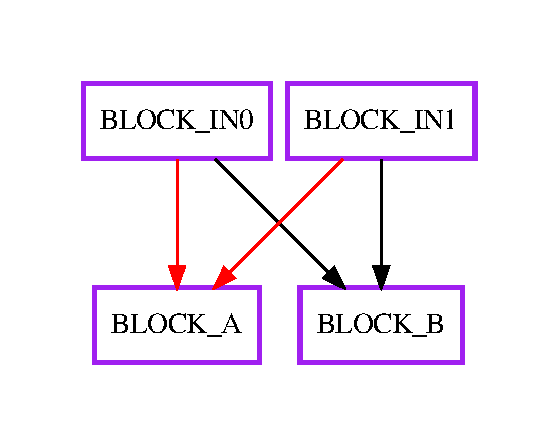
\includegraphics{TestPattern/static_basic.pdf}
        \caption{Pattern for the static basic test}
        \label{fig:Pattern_for_the_static_basic_test}
    \end{figure}
	\item Success Criteria

	The test is successful if no pattern is loaded. Checked with \texttt{dm-sched status}
\end{enumerate}
\subsection{Coupling}
\begin{enumerate}
	\item Purpose of Test

	This test enlarges an existing pattern with a second pattern with edges into the first 
	pattern. See Figure~\ref{fig:Pattern_for_the_static_coupling_test} for the test patterns.
	\item Test Actions

	First, a pattern with three nodes is added. In a second step a pattern with additional three nodes is added. 
	This pattern contains edges into the first pattern.
    \begin{figure}
        \centering 
        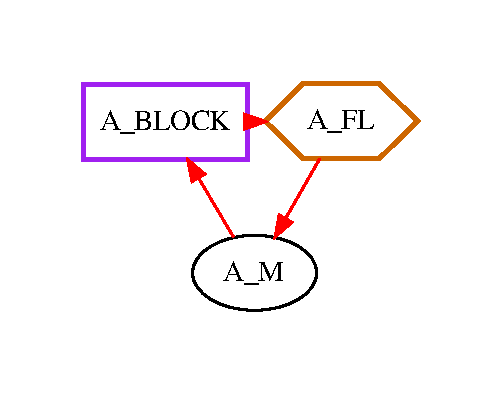
\includegraphics{TestPattern/static_coupling1.pdf}
        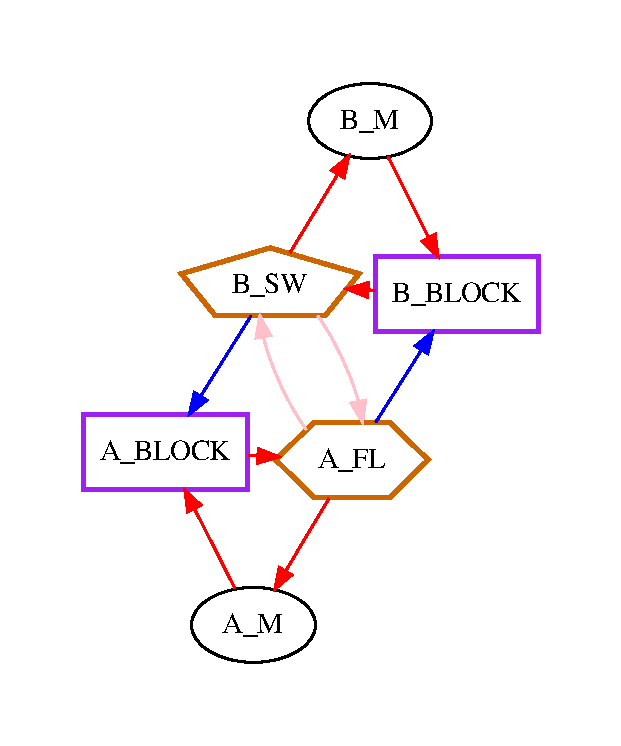
\includegraphics{TestPattern/static_coupling2.pdf}
        \caption{Pattern for the static coupling test before and after coupling}
        \label{fig:Pattern_for_the_static_coupling_test}
    \end{figure}
	\item Success Criteria

	After adding the two patterns the status is checked with \texttt{dm-sched status}. The resulting \texttt{download.dot} is 
	compared to an expected dot-file.
\end{enumerate}
\subsection{Priority and Type}
\begin{enumerate}
	\item Purpose of Test

The test check the relative and the absolute time values for two nodes in a four node pattern. 
See Figure~\ref{fig:Pattern_for_the_static_priority_and_type_test} for the test pattern 
and \ref{fig:Pattern_for_the_static_priority_and_type_test_with_meta_nodes} for the test pattern with meta nodes, 
displaying the priority queues.
	\item Test Actions

	Add the pattern, check the relative time values. Clear the data master. Add the pattern again and check the absolute time values.
    \begin{figure}
        \centering 
        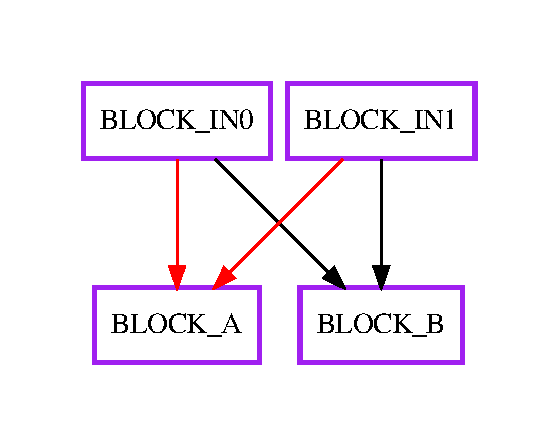
\includegraphics{TestPattern/static_prio_and_type.pdf}
        \caption{Pattern for the static priority and type test}
        \label{fig:Pattern_for_the_static_priority_and_type_test}
    \end{figure}
    \begin{figure}
        \centering 
        \includegraphics*[height=0.95\textheight,keepaspectratio]{TestPattern/static_prio_and_type_meta.pdf}
        \caption{Pattern for the static priority and type test with meta nodes}
        \label{fig:Pattern_for_the_static_priority_and_type_test_with_meta_nodes}
    \end{figure}
	\item Success Criteria

	Two checks of the time values with \texttt{dm-cmd rawqueue}.
\end{enumerate}
\section{Dynamic Tests}
\subsection{Async}
\begin{enumerate}
	\item Purpose of Test

	See Figure~\ref{fig:Pattern_for_the_dynamic_async_test} for the test pattern.
	\item Test Actions
    \begin{figure}
        \centering 
        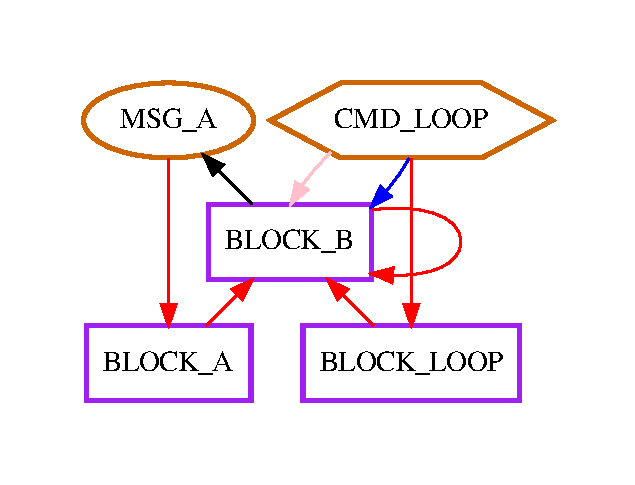
\includegraphics{TestPattern/dynamic_async.pdf}
        \caption{Pattern for the dynamic async test}
        \label{fig:Pattern_for_the_dynamic_async_test}
    \end{figure}
	\item Success Criteria
\end{enumerate}
\subsection{Basic}
\subsubsection{Run CPU 0 single}
\begin{enumerate}
	\item Purpose of Test

	See Figure~\ref{fig:Pattern_for_the_dynamic_run_CPU_0_single_test} for the test pattern.
	\item Test Actions
    \begin{figure}
        \centering 
        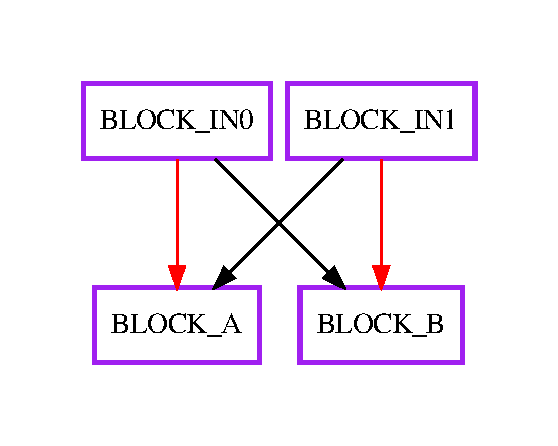
\includegraphics{TestPattern/dynamic_basic_run_cpu0_single.pdf}
        \caption{Pattern for the dynamic run CPU 0 single test}
        \label{fig:Pattern_for_the_dynamic_run_CPU_0_single_test}
    \end{figure}
	\item Success Criteria
\end{enumerate}
\subsubsection{Run all single}
\begin{enumerate}
	\item Purpose of Test

	See Figure~\ref{fig:Pattern_for_the_dynamic_run_all_test} for the test pattern.
	\item Test Actions
    \begin{figure}
        \centering 
        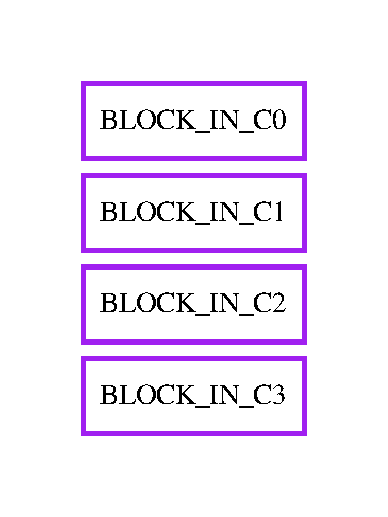
\includegraphics{TestPattern/dynamic_basic_run_all_single.pdf}
        \caption{Pattern for the dynamic run all test}
        \label{fig:Pattern_for_the_dynamic_run_all_test}
    \end{figure}
	\item Success Criteria
\end{enumerate}
\subsubsection{Start Stop Abort}
\begin{enumerate}
	\item Purpose of Test

	See Figure~\ref{fig:Pattern_for_the_dynamic_start_stop_abort_test} for the test pattern.
	\item Test Actions
    \begin{figure}
        \centering 
        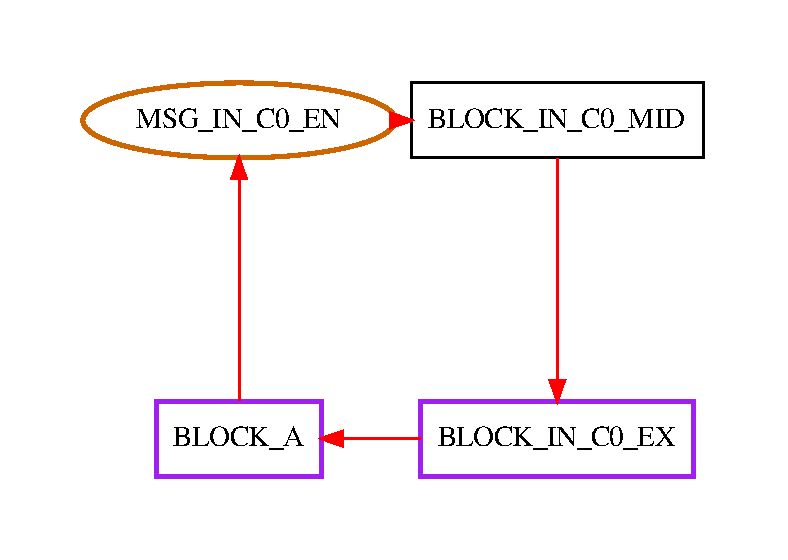
\includegraphics{TestPattern/dynamic_basic_start_stop_abort.pdf}
        \caption{Pattern for the dynamic start stop abort test}
        \label{fig:Pattern_for_the_dynamic_start_stop_abort_test}
    \end{figure}
	\item Success Criteria
\end{enumerate}
\subsection{Branch}
\subsubsection{Single}
\begin{enumerate}
	\item Purpose of Test

	See Figure~\ref{fig:Pattern_for_the_dynamic_branch_single_test} for the test pattern.
	\item Test Actions
    \begin{figure}
        \centering 
        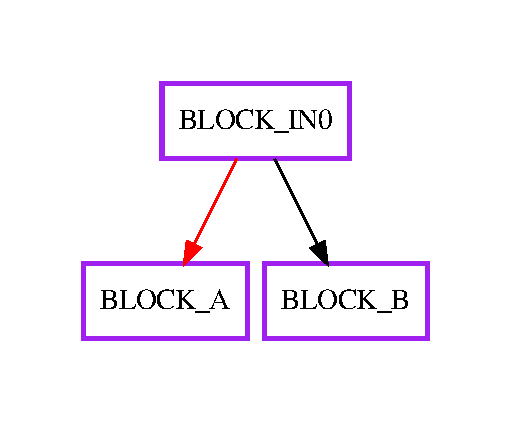
\includegraphics{TestPattern/dynamic_branch_single.pdf}
        \caption{Pattern for the dynamic branch single test}
        \label{fig:Pattern_for_the_dynamic_branch_single_test}
    \end{figure}
	\item Success Criteria
\end{enumerate}
\subsection{Coupling}
\begin{enumerate}
	\item Purpose of Test

	Test not working, needs set up.
	\item Test Actions
	\item Success Criteria
\end{enumerate}
\subsection{Loop}
\begin{enumerate}
	\item Purpose of Test

	See Figure~\ref{fig:Pattern_for_the_dynamic_loop_test} for the test pattern.
	\item Test Actions
    \begin{figure}
        \centering 
        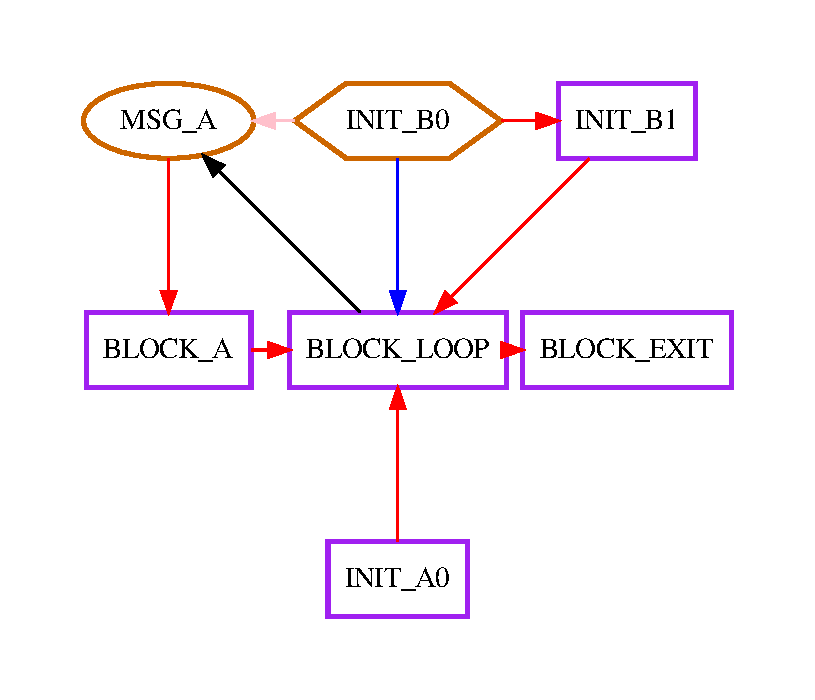
\includegraphics{TestPattern/dynamic_loop.pdf}
        \caption{Pattern for the dynamic loop test}
        \label{fig:Pattern_for_the_dynamic_loop_test}
    \end{figure}
	\item Success Criteria
\end{enumerate}
\subsection{Switch}
\begin{enumerate}
	\item Purpose of Test

	Test not working, needs set up.
	\item Test Actions
	\item Success Criteria
\end{enumerate}
\end{document}
